\section{Source of Adaptivity}\label{subsec:adaptivity}
To understand why the proposed method shows advantages in achieving better learning performance in the challenging scenario of performing dynamic locomotion skills with varying environment parameters, we delve into an examination of the latent representation provided by the encoder for long I/O history, as shown in Fig.~\ref{fig:latent_vis} and Appnedix~\ref{appendix:walking_latent}.
These results are obtained in simulation. 
As we will see, the encoder that utilizes long I/O history can capture both time-varying events and time-invariant changes in dynamics parameters in all the locomotion skills we developed. 


\begin{figure*}[!htp]
\centering
\begin{subfigure}{0.66\linewidth}
  \centering
  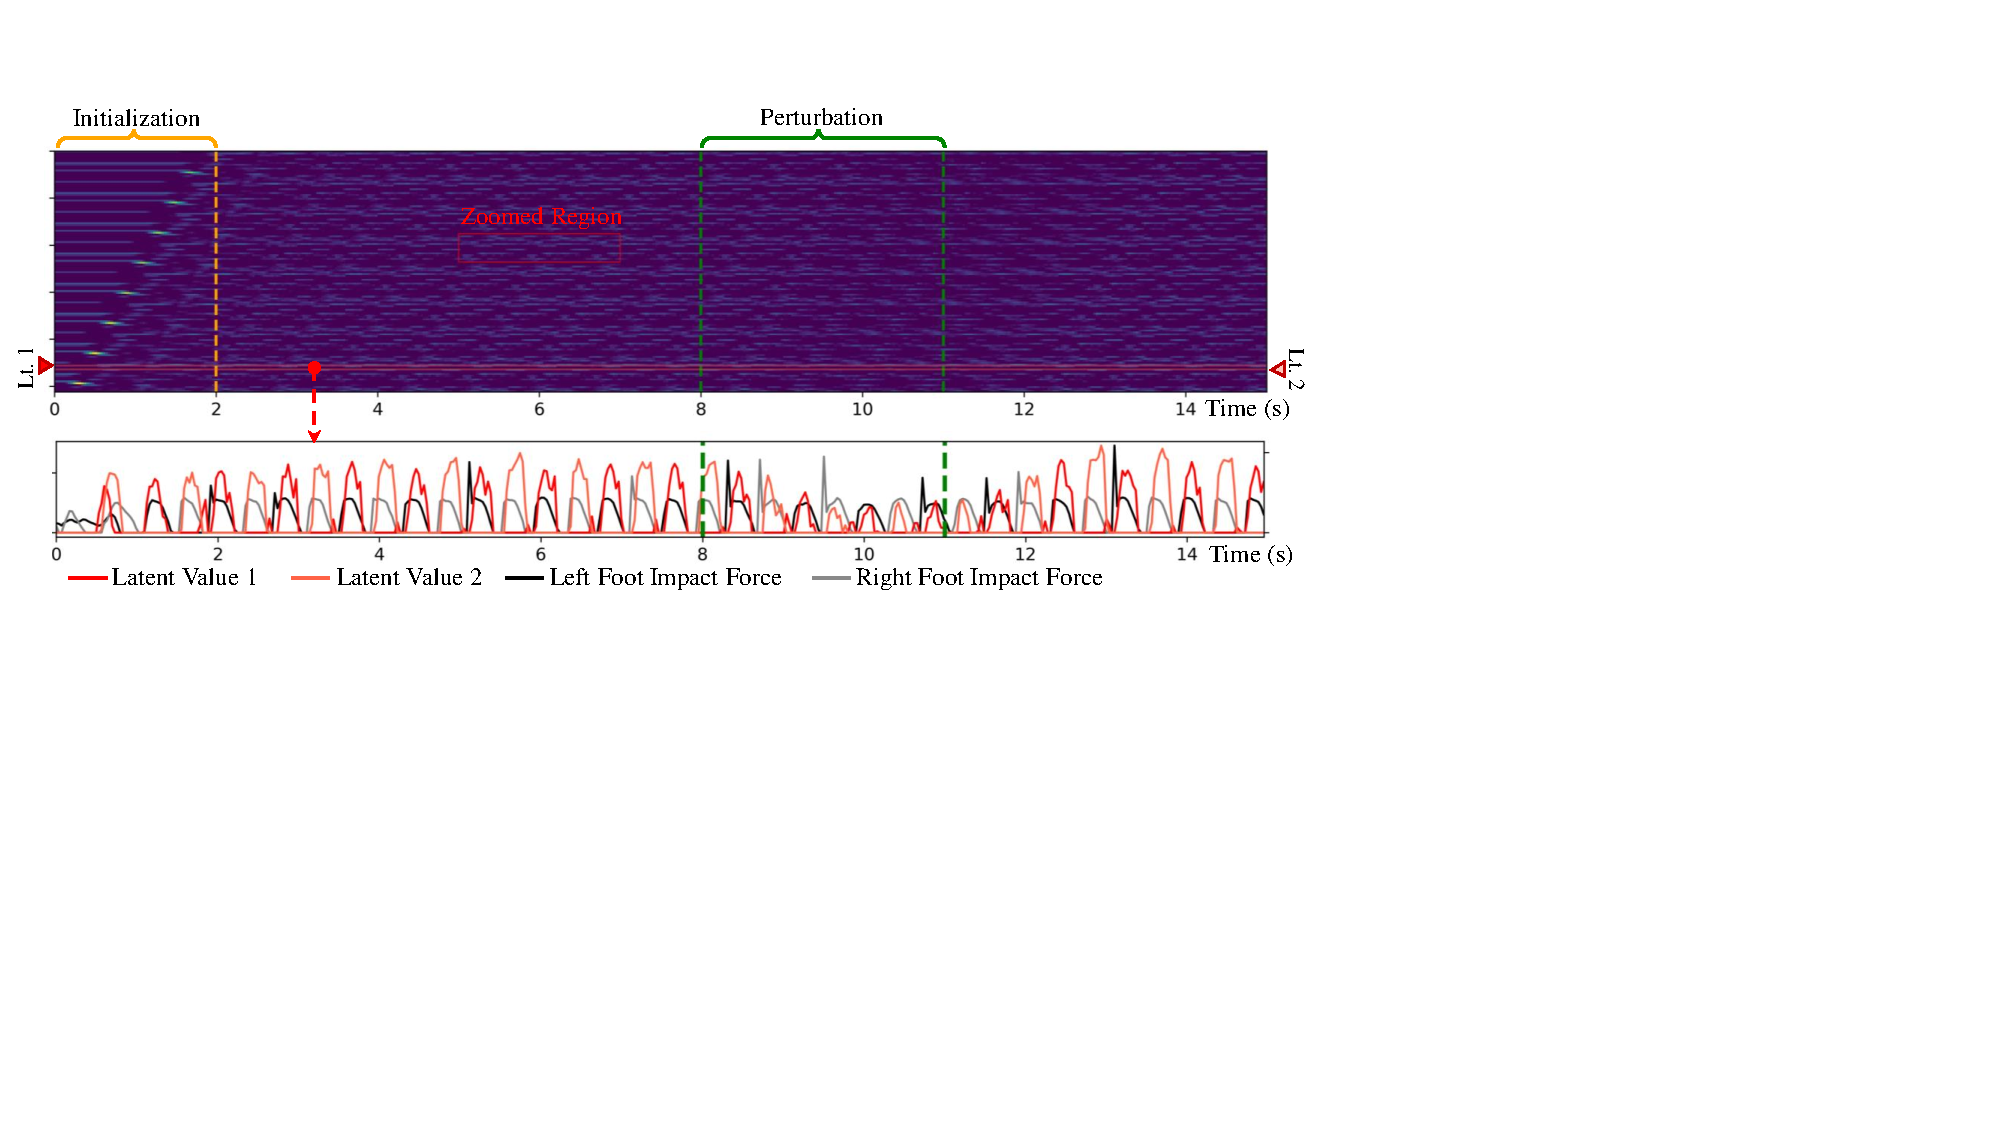
\includegraphics[width=\linewidth]{figures/latent_run_force.pdf}
  \caption{(Top) Recorded latent representation after long-term I/O history encoder during \underline{running}. (Bottom) Comparison of two selected dimensions (marked as red lines in the top plot) with recorded impact forces on each of the robot's feet.}
  \label{subfig:latent_run_force}
\end{subfigure}
\begin{subfigure}{0.33\linewidth}
  \centering
  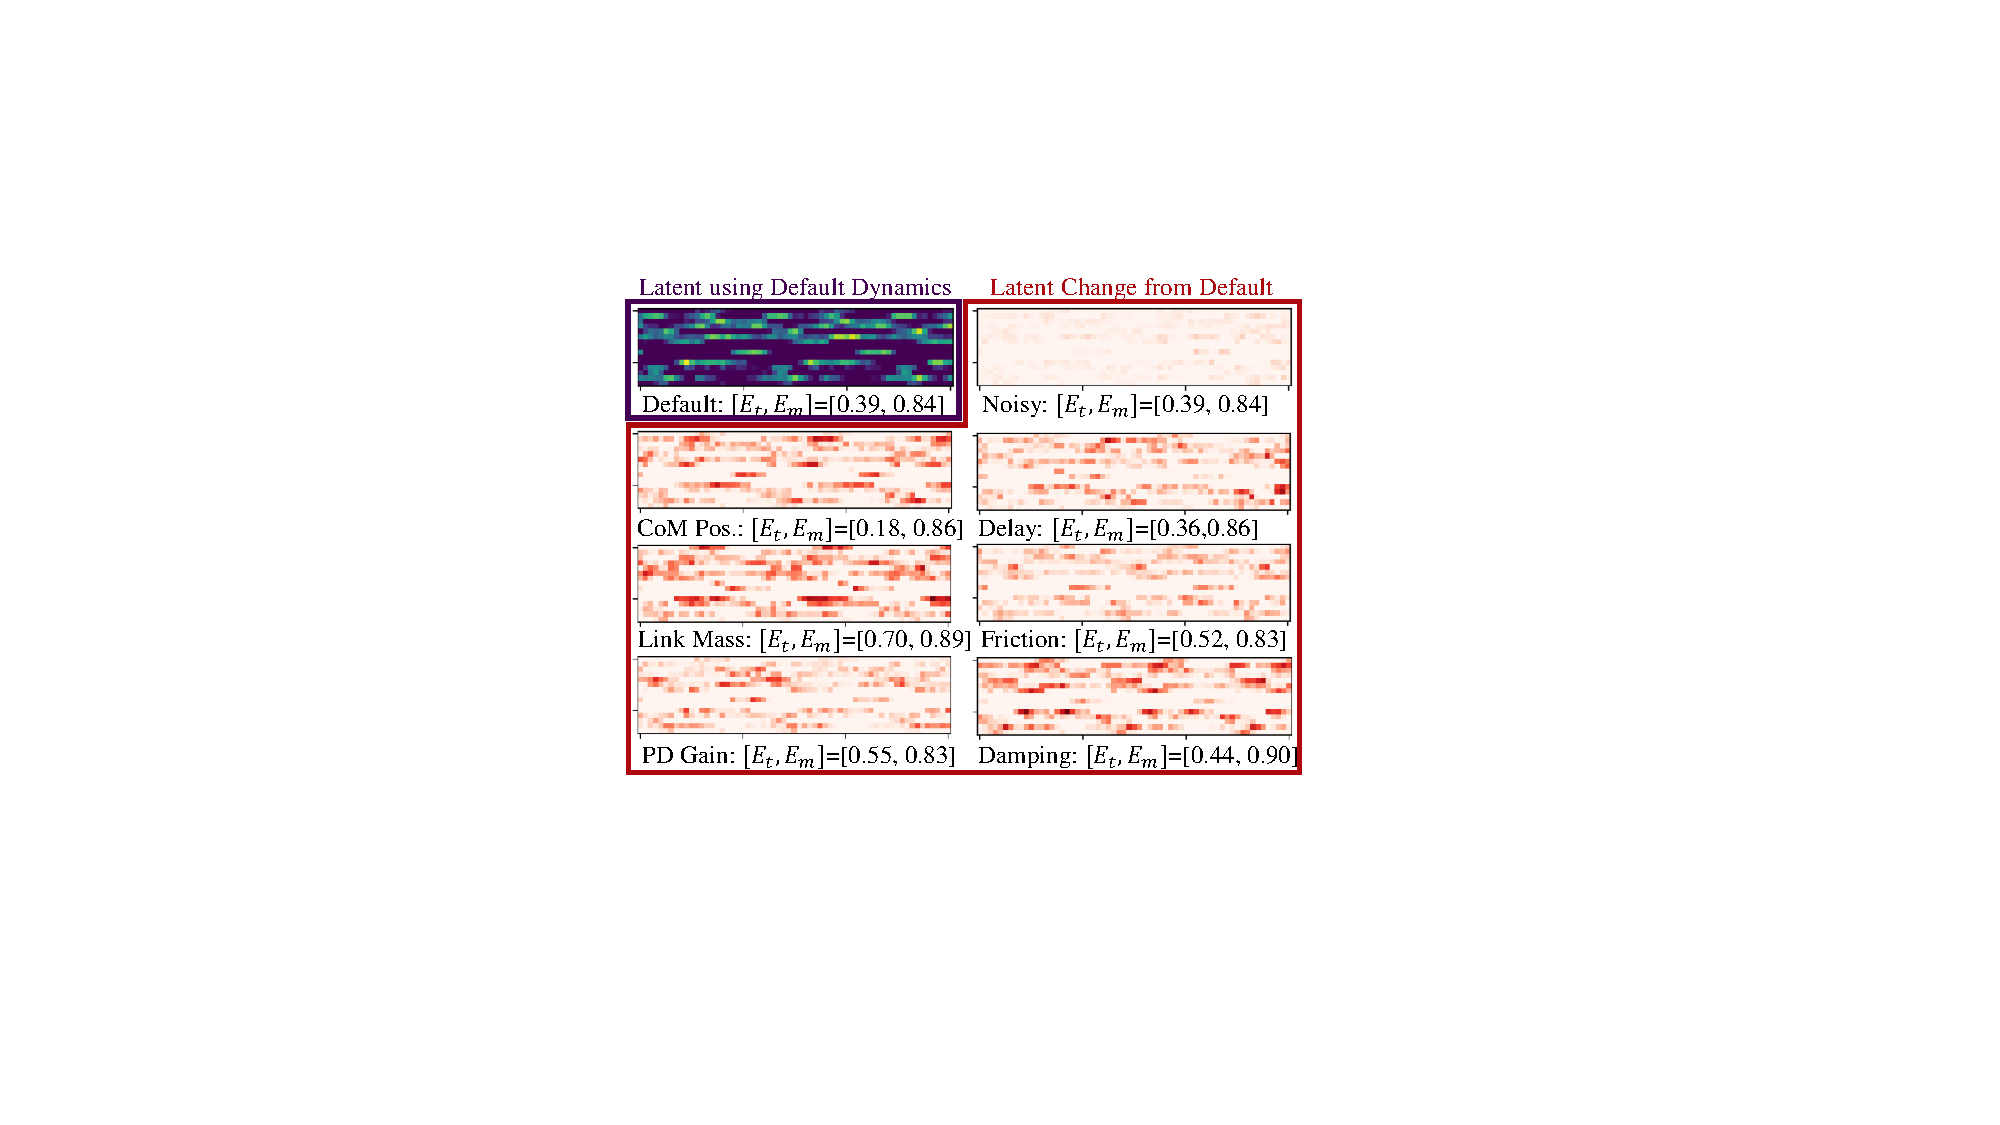
\includegraphics[width=\linewidth]{figures/latent_run_zoomed_delta.pdf}
  \caption{The blue plot shows the robot's latent representation with default dynamics parameters during running. The red plots indicate changes in the same region under different dynamics.}
  \label{subfig:latent_run_zoomed}
\end{subfigure}

\begin{subfigure}{0.66\linewidth}
  \centering
  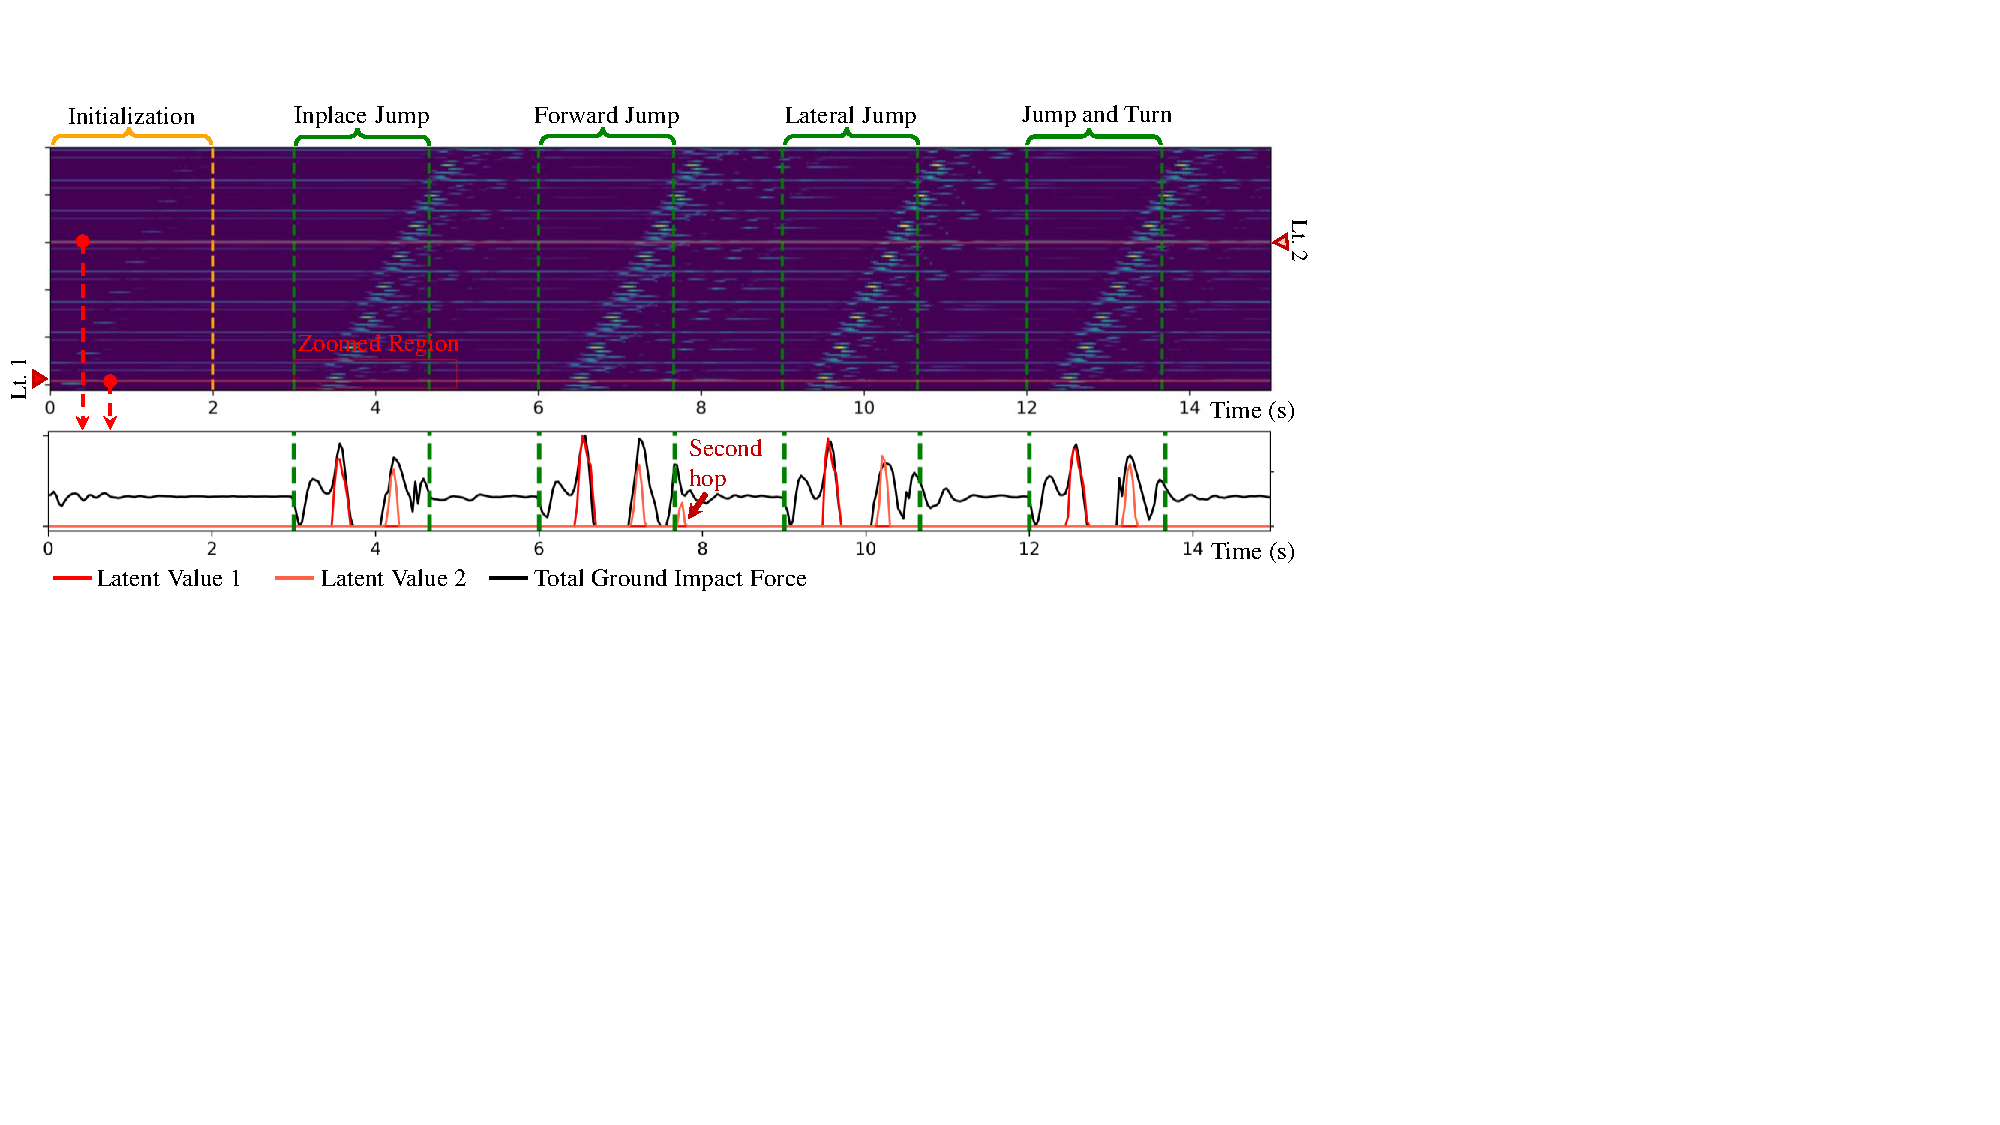
\includegraphics[width=\linewidth]{figures/latent_jump_force.pdf}
  \caption{(Top) Recorded latent representation after long-term I/O history encoder during \underline{jumping}. (Bottom) Comparison of two selected dimensions (marked as red lines in the top plot) with recorded total impact forces on both of the robot's two feet.}
  \label{subfig:latent_jump_force}
\end{subfigure}
\begin{subfigure}{0.33\linewidth}
  \centering
  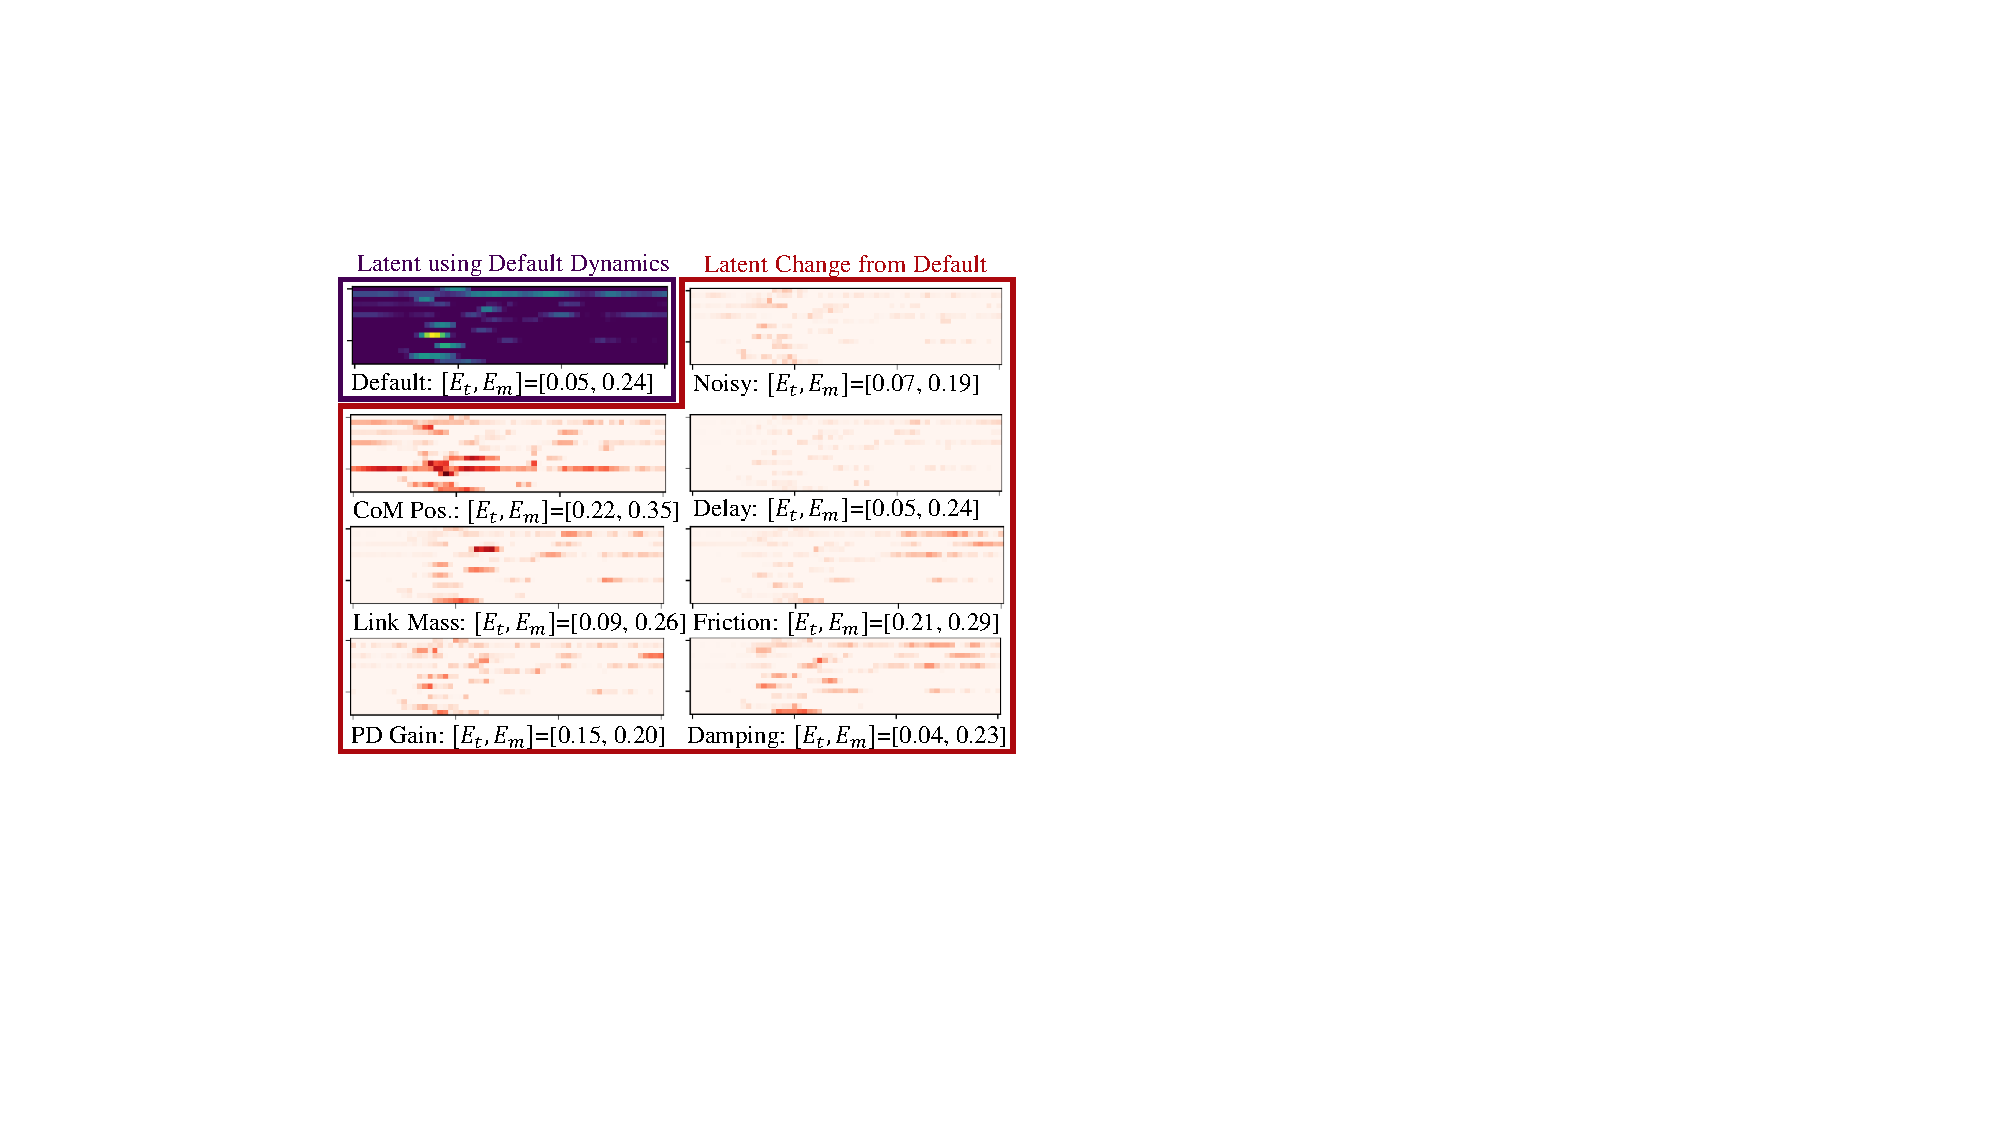
\includegraphics[width=\linewidth]{figures/latent_jump_zoomed_delta.pdf}
  \caption{The blue plot shows the robot's latent representation with default dynamics parameters during jumping. The red plots indicate changes in the same region under different dynamics.}
  \label{subfig:latent_jump_zoomed}
\end{subfigure}
\caption{Adaptivity test in simulation (MuJoCo). We evaluate the latent representation profiles from the output of the long-term I/O history encoder during bipedal running (Fig.~\ref{subfig:latent_run_force}) and jumping (Fig.~\ref{subfig:latent_jump_force}) where lighter color represents a larger relative value. 
After the initialization of the history encoder (first 2 seconds), variations in the latent embedding are noticeable for different activities like running versus jumping or standing, for specific jumping targets, and for the existence of external perturbations. Two latent values (indicated by red horizontal lines in the top plots) are plotted in the bottom plots to show thta the latent space also captures the changes in the impact forces.  
To conduct an ablation study on time-invariant dynamics parameters, we examine the same regions inside red boxes (titled zoomed region) in Fig.~\ref{subfig:latent_run_force},~\ref{subfig:latent_jump_force} and show these regions in Fig.~\ref{subfig:latent_run_zoomed},~\ref{subfig:latent_jump_zoomed} when the robot is performing constant-speed running and in-place jumping respectively. 
The \emph{Latent using Default Dynamics} shows these regions when then robot's nominal model is simulated without any changes to the dynamics or introducing noise or delays. The \emph{Latent Change from Default} shows the delta change in the same regions when we adjust the CoM position of each link (marked as \textit{CoM Pos}), link mass (\textit{Link Mass}), PD gains used on each motor (\textit{PD Gain}), ground friction (\textit{Friction}), joint damping ratio (\textit{Damping}), communication delay (\textit{Delay}), and noise levels (\textit{Noisy}) one at the time.  
In these plots, a larger change is represented by a darker color. This shows that the latent embedding can reflect different changes in dynamics, while effectively filtering out noise which causes little changes. 
Despite significant environment changes, control performance metrics like task completion error ($E_t$) and motion tracking error ($E_m$) show minor degradation, showcasing adaptivity to dynamic changes using the proposed controller. We further visualize the corresponding saliency map in Appendix.~\ref{appendix:saliency}.}
\label{fig:latent_vis}
\end{figure*}



\subsection{Time Varying Embedding}
In this subsection, we observe that the latent embedding from the long I/O history encoder can effectively adapt to time-varying external disturbances or locomotion tasks, implicitly estimating contact events and/or external forces across all three distinct locomotion skills.
\paragraph{Periodic Running}
Using the running policy obtained by the proposed method, we recorded the latent embedding over a 15-second duration, initiating from a standing position and progressing to follow the constant running speed command of 3 m/s. 
A persistent backward perturbation force of 40 N was applied to the robot base from 8 to 11 seconds. 
The evolution of latent values over time is depicted in Fig.~\ref{subfig:latent_run_force}.

Given that running is a periodic skill, the latent embedding also exhibits a periodic pattern once the gait has stabilized, as seen in Fig.~\ref{subfig:latent_run_force} after 2 seconds. 
Additionally, the presence of the perturbation introduces variations in the latent embedding (within the green dashed lines), showcasing the capability to capture time-varying disturbances. 

Additionally, we found two intriguing latent dimensions highlighted by the red line and plots in Fig.~\ref{subfig:latent_run_force}. 
These two latent signals exhibit a strong correlation with the impact force on the robot's left and right foot. 
Specifically, the values of these two latent dimensions vary in a tendency consistent with the ground truth impact force recorded in simulation, reaching zero when the corresponding force is zero (the respective foot is in a swing phase).
This result highlights a crucial and demanding capability for controlling legged robots: contact estimation, as the trajectory breaks upon contact. 

The advantage of implicit contact estimation becomes more evident with changes in these two latent dimensions in the presence of external perturbation (shown within the green dashed lines in Fig.~\ref{subfig:latent_run_force}). 
Despite the unchanged magnitude of the ground impact force, these two latent values shift to a lower envelope during the perturbation, followed by a recovery to the previous envelope after the perturbation is taken out. 
While an exact explanation for this change remains elusive as it is learned purely through data, it \emph{may} be attributed to the notion that both external perturbation and ground reaction force can be treated as a generalized external force $\bm{\zeta}_{\text{ext}}$ applied to the robot, as implied by the robot's full-order dynamics \eqref{eq:full_order_dynamics}. 
The robot may have unconsciously learned to embed such external forces all together into these signals and leverage them in control, without explicit human engineering, through the provided long I/O history. 
A similar capacity for such a long history encoder for periodic walking skill is also observed, and we analyze it briefly in Appendix~\ref{appendix:walking_latent}.  

\paragraph{Aperiodic Jumping}
Despite the periodic running and walking skills, we also discovered a similar capacity of the I/O history encoder to capture time-varying information in aperiodic skills like jumping. 
As depicted in Fig.~\ref{subfig:latent_jump_force}, Cassie was commanded to execute different jumping tasks every 3 seconds, starting from an in-place jump to a 1.4-meter forward jump, followed by a 0.5-meter sideways jump and a jump and turn of $-60^\circ$ before standing. 

The recorded time-evolving latent representation reveals a distinct contrast between jumping phases (that have more varying and non-zero signals) and standing phases (with less varying signals). 
Furthermore, for different jumping tasks, the latent values during the jumping phases differ, as illustrated in Fig.~\ref{subfig:latent_jump_force}.

Moreover, we discovered two latent dimensions that strongly correlate with contact events during jumping, as indicated by the red lines and plotted in Fig.~\ref{subfig:latent_jump_force}. 
In contrast to a common human expectation for a single binary variable of contact during jumping (either in contact or not), the robot learned to utilize two distinct signals: take-off event and landing event, estimated by Latent Value 1 and 2, respectively, as depicted in Fig.~\ref{subfig:latent_jump_force}. 
For example, the Latent Value 1 begins to increase and drops to zero just before the total contact force reaches zero (indicating the robot is starting to take off), while Latent Value 2 only becomes active at the moment the robot lands. 
Furthermore, during the forward jump the robot executes a small hop after it lands, Latent Value 2 exhibits an additional spike during that additional hop.
Such separated signals for take-off and landing could provide more informative cues for controlling a bipedal jumping skill, given the difference in control complexity during the flight and landing phases.


\subsection{Adaptive Embedding for Changes in Dynamics}
We now assess how the latent embedding changes with (time-invariant) variations in the robot dynamics model, specifically, alterations in the $\mathbf{M}$, $\mathbf{C}$, $\mathbf{G}$, $\bm{\kappa}$, and Jacobians in~\eqref{eq:full_order_dynamics}, or with corrupted measurements (including noise and delays).
Using the aforementioned running policy, we focus on a segment of the periodic pattern illustrated in Fig.~\ref{subfig:latent_run_force}, highlighted by the red block. 
The zoomed-in pattern, observed when controlling the robot with the default dynamics model, is visualized in Fig.~\ref{subfig:latent_run_zoomed}. 

We conduct an ablation study using the same running policy in the same task (tracking a 3 m/s command) with changes in the dynamics parameters.
In particular, we adjust one specific modeling parameter one at time, such as the link CoM position (increased by $8$ cm for all links), link mass ($30\%$ greater for all links), joint damping ratio (8 times the default value), and PD gains used on each motor ($40\%$ higher than the default value), and lower ground friction (static friction ratio set to 0.5 for slippery ground). 
As shown in Fig.~\ref{subfig:latent_run_zoomed}, each change of these dynamics parameters results in a significant shift in the resulting latent embedding compared to the pattern obtained with the default model.
However, evaluating control performance metrics, such as task completion (tracking error $E_t$ between the robot's actual speed and desired speed) and motion tracking (motion deviation $E_m$ from the robot's actual motor position and reference motion), reveals minimal change. 

A similiar ablation study is undertaken in jumping and walking skills, recorded in Fig.~\ref{subfig:latent_jump_zoomed} and Appendix~\ref{appendix:walking_latent}, respectively.
Specifically, within the in-place jumping task utilizing the obtained jumping policy, we modify the same dynamics parameters as in running, resulting in varying patterns of the latent embedding for different dynamics models.
Despite these alterations, the control performance metrics, such as task completion $E_t$ (the error in the landing position compared to the desired one) and motion tracking error $E_m$, also show minimal changes.

When assessing the influence of corrupted measurements on the latent embedding, the latency in control and observation (0.025 s) induced noticeable changes in running and walking, as showcased in Fig.~\ref{subfig:latent_run_zoomed} and Fig.~\ref{subfig:latent_walk_zoomed}. 
Surprisingly, the introduction of significantly larger noise (2 times larger than the upper bound used during training as listed in Table~\ref{tab:randomization}) does not exert a considerable effect on the resulting latent embedding for all running, jumping, and walking skills. 
This result underscores the efficacy of the long history encoder in effectively filtering out the added zero-mean noise, which may be also brought by the CNN structure. 

\subsection{Summary of Results}
This ablation study highlights the adaptivity of the proposed controller. 
Empowered by the history encoder's ability to capture meaningful information from the I/O history, this controller can adapt to time-varying events such as external perturbations or contacts, time-invariant changes in dynamics parameters, and filter out measurement noise, and therefore, effectively execute the control task with minimal performance degradation. 
This capability explains why the proposed structure excels in the challenging training setting with a large range of randomization of dynamics parameters.
Notably, in order to fully harness such advantages brought by the robot's long I/O history, a proper structure (dual-history approach) and training strategy (end-to-end training) are necessary, as discussed in Sec.~\ref{sec:policy_structure}.
